\begin{tikzpicture}[remember picture,overlay,x=1cm,y=1cm]
\begin{scope}[shift={(current page.south west)}]
  \fill[Navy] (0,0) rectangle (16,9);

  % Primary visual: real plant context, kept quiet so the title owns the slide.
  \begin{scope}
    \clip (9.25,0) rectangle (16,9);
    \node[anchor=center] at (12.55,4.55) {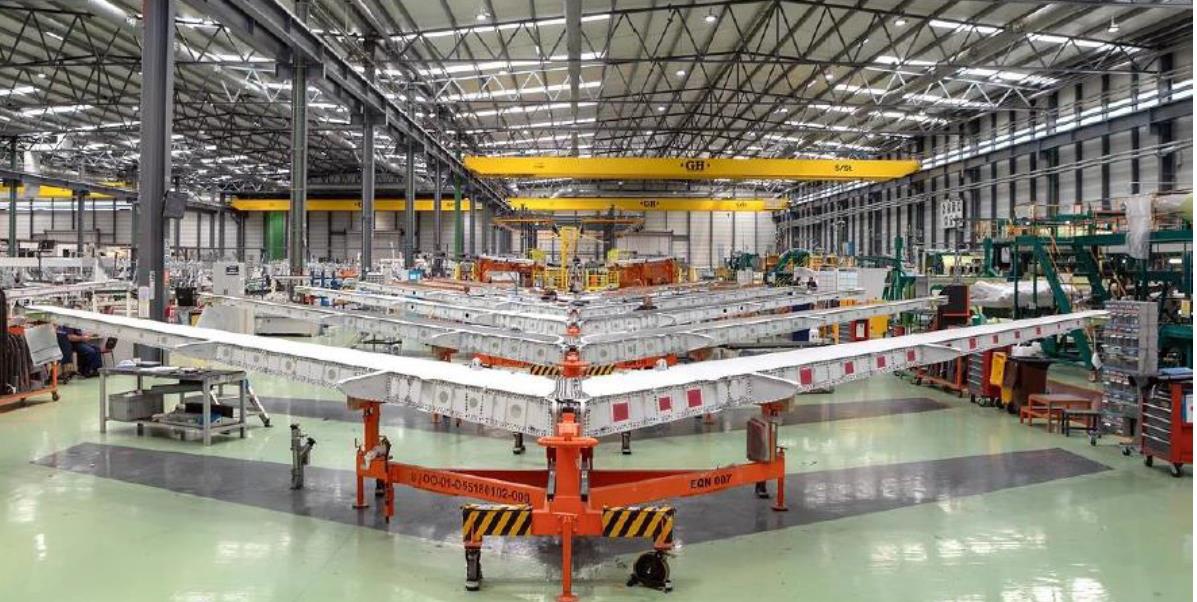
\includegraphics[height=9.25cm]{../figures/source/alestis_htp_nave.png}};
    \fill[Navy2,opacity=0.50] (9.25,0) rectangle (16,9);
  \end{scope}
  \draw[Cyan,line width=1.0pt] (9.25,0.72) -- (9.25,8.34);

  \node[anchor=west,font=\fontsize{7.2}{8.0}\selectfont\bfseries,text=Cyan] at (0.88,7.94) {LUNABOTICS \textbullet{} OFERTA T\'ECNICA Y COMERCIAL};
  \node[anchor=east] at (15.25,8.24) {
\includegraphics[width=1.34cm]{../images/logo-viu-w.png}};

  \node[anchor=west,font=\fontsize{25.5}{27.0}\selectfont\bfseries,text=white,text width=8.10cm,align=left] at (0.86,6.70) {Sistema\\AMR-FOD-Kitting};
  \node[anchor=west,font=\fontsize{12.0}{13.5}\selectfont\bfseries,text=white!82,text width=7.70cm,align=left] at (0.92,4.72) {Automatizaci\'on intralog\'istica para HTP A320 y secci\'on 19.1};
  \draw[Cyan,line width=1.15pt] (0.94,4.06) -- (4.92,4.06);

  \node[anchor=west,font=\fontsize{7.2}{8.4}\selectfont,text=white!78,text width=7.25cm,align=left] at (0.94,3.18) {Actividad 1 \textbullet{} Sistemas Rob\'oticos M\'oviles\\Profesor: Jos\'e I. I\~niguez\\Autor: Jorge Luis Mayorga Taborda\\Entrega: 26 de mayo de 2026};

  \node[anchor=west,font=\fontsize{6.6}{7.5}\selectfont\bfseries,text=Cyan] at (0.94,1.36) {TESIS};
  \node[anchor=west,font=\fontsize{8.2}{9.3}\selectfont\bfseries,text=white,text width=6.95cm,align=left] at (0.94,0.88) {Medir un piloto AMR antes de escalar la flota.};

  \fill[white,opacity=0.92,rounded corners=5pt] (9.88,1.78) rectangle (14.55,3.42);
  \draw[Amber,line width=0.55pt,rounded corners=5pt] (9.88,1.78) rectangle (14.55,3.42);
  \node[anchor=west,font=\fontsize{6.1}{6.9}\selectfont\bfseries,text=Amber] at (10.16,3.08) {CASO PILOTO};
  \node[anchor=west,font=\fontsize{12.0}{13.0}\selectfont\bfseries,text=Navy] at (10.16,2.58) {HTP A320 · 19.1};
  \node[anchor=west,font=\fontsize{6.2}{7.1}\selectfont,text=Ink,text width=3.92cm] at (10.18,2.08) {Kits, RFID/QR, registro de entregas e inspecci\'on FOD.};

  \node[anchor=west,font=\fontsize{5.4}{6.1}\selectfont,text=white!72,text width=3.82cm,align=left] at (9.88,0.94) {Foto base: Alestis HTP. Propuesta MROB-VIU 2026.};

  \webcamplaceholder
\end{scope}
\end{tikzpicture}
